% Appendix B: Counterexample — Balanced Ternary Tree on n=8

We present the full computation showing that Construction~A fails on
the balanced ternary tree with $n = 8$.

\subsection*{Tree structure}

The balanced ternary tree on 8 nodes has root label~4 and the
following adjacency:
\begin{center}
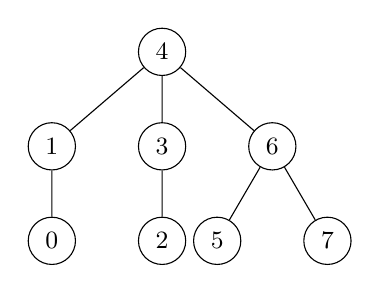
\begin{tikzpicture}[
  level distance=12mm, sibling distance=14mm,
  every node/.style={circle,draw,minimum size=6mm,inner sep=0pt,
    font=\small}
]
\node {4}
  child { node {1}
    child { node {0} }
  }
  child { node {3}
    child { node {2} }
  }
  child { node {6}
    child { node {5} }
    child { node {7} }
  };
\end{tikzpicture}
\end{center}

This tree has depth~2 and is \emph{not} a star.

\subsection*{Index sets from Construction~A}

Applying the generic tree-derived formula~\eqref{eq:tree-derived-sets}:
\begin{center}
\begin{tabular}{@{}clll@{}}
\toprule
$j$ & $\Uset{j}$ & $P(j)$ & $\Occ{j}$ \\
\midrule
0 & $\{1, 4\}$       & $\emptyset$     & $\{0\}$ \\
1 & $\{4\}$           & $\{0\}$         & $\{0, 1\}$ \\
2 & $\{3, 4\}$       & $\{1\}$         & $\{2\}$ \\
3 & $\{4\}$           & $\{1, 2\}$     & $\{2, 3\}$ \\
4 & $\emptyset$       & $\{1, 3\}$     & $\{0,1,2,3,4,5,6,7\}$ \\
5 & $\{6, 4\}$       & $\{1, 3\}$     & $\{5\}$ \\
6 & $\{4\}$           & $\{1, 3, 5\}$ & $\{5, 6, 7\}$ \\
7 & $\{6, 4\}$       & $\{1, 3, 5\}$ & $\{7\}$ \\
\bottomrule
\end{tabular}
\end{center}

\subsection*{Majorana operators (partial)}

From these index sets, the Majorana operators for modes 4 and~7 are:
\begin{align*}
  c_4 &= -Y_1 Y_3 X_4 Z_5 Z_6 Z_7, \\
  d_4 &= Y_1 Y_3 Y_4 Z_5 Z_6 Z_7, \\
  c_7 &= -Y_1 Y_3 Y_5 X_6 X_7, \\
  d_7 &= Y_1 Y_3 Y_5 X_6 Y_7.
\end{align*}
(Operators on unlisted qubits are identity.)

\subsection*{Failed anticommutator}

Computing $\acomm{\an{4}}{\ad{7}}$, where
$\an{4} = \tfrac{1}{2}(c_4 + i\,d_4)$ and
$\ad{7} = \tfrac{1}{2}(c_7 - i\,d_7)$:

\begin{align*}
  \acomm{\an{4}}{\ad{7}}
    &= \tfrac{1}{4}\bigl[
      \acomm{c_4}{c_7} + i\,\acomm{d_4}{c_7}
      - i\,\acomm{c_4}{d_7} + \acomm{d_4}{d_7}
    \bigr].
\end{align*}

For a valid encoding, this should vanish ($4 \neq 7$).  Instead:
\begin{align*}
  \acomm{c_4}{c_7} &= -2\,ZZZZZIZZ, \\
  \acomm{d_4}{d_7} &= +2\,ZZZZZIZZ, \\
  \acomm{c_4}{d_7} &= -2i\,ZZZZZIZZ, \\
  \acomm{d_4}{c_7} &= -2i\,ZZZZZIZZ.
\end{align*}

These do \emph{not} cancel:
\begin{equation*}
  \acomm{\an{4}}{\ad{7}} = (0.5i)\; ZZZZZIXY + (-0.5)\; ZZZZZIXX
    \neq 0.
\end{equation*}

\subsection*{Diagnosis}

The failure matches the structural mechanism of
\cref{thm:star-tree}: node~6 is not a star root, and the
depth-2 path $4 \to 6 \to 7$ triggers the symmetric-difference
cancellation that assigns identity to the middle node, producing an
even number of anticommuting positions.

\subsection*{Verification by Construction~B}

Applying Construction~B (path-based encoding, \cref{sec:tree-encoding})
to the \emph{same} balanced ternary tree produces Majorana operators
that satisfy \emph{all} $\binom{16}{2} = 120$ anticommutation
relations exactly.  The tree topology is not the problem; the
index-set derivation method is.
